\documentclass{article}
\usepackage[paperwidth=290mm,paperheight=80mm,margin=3mm]{geometry}
\usepackage{tikz}
\usepackage{amsmath}
\usetikzlibrary{arrows.meta,positioning,shapes.geometric,fit,backgrounds,calc}
\pagestyle{empty}

\begin{document}
\noindent
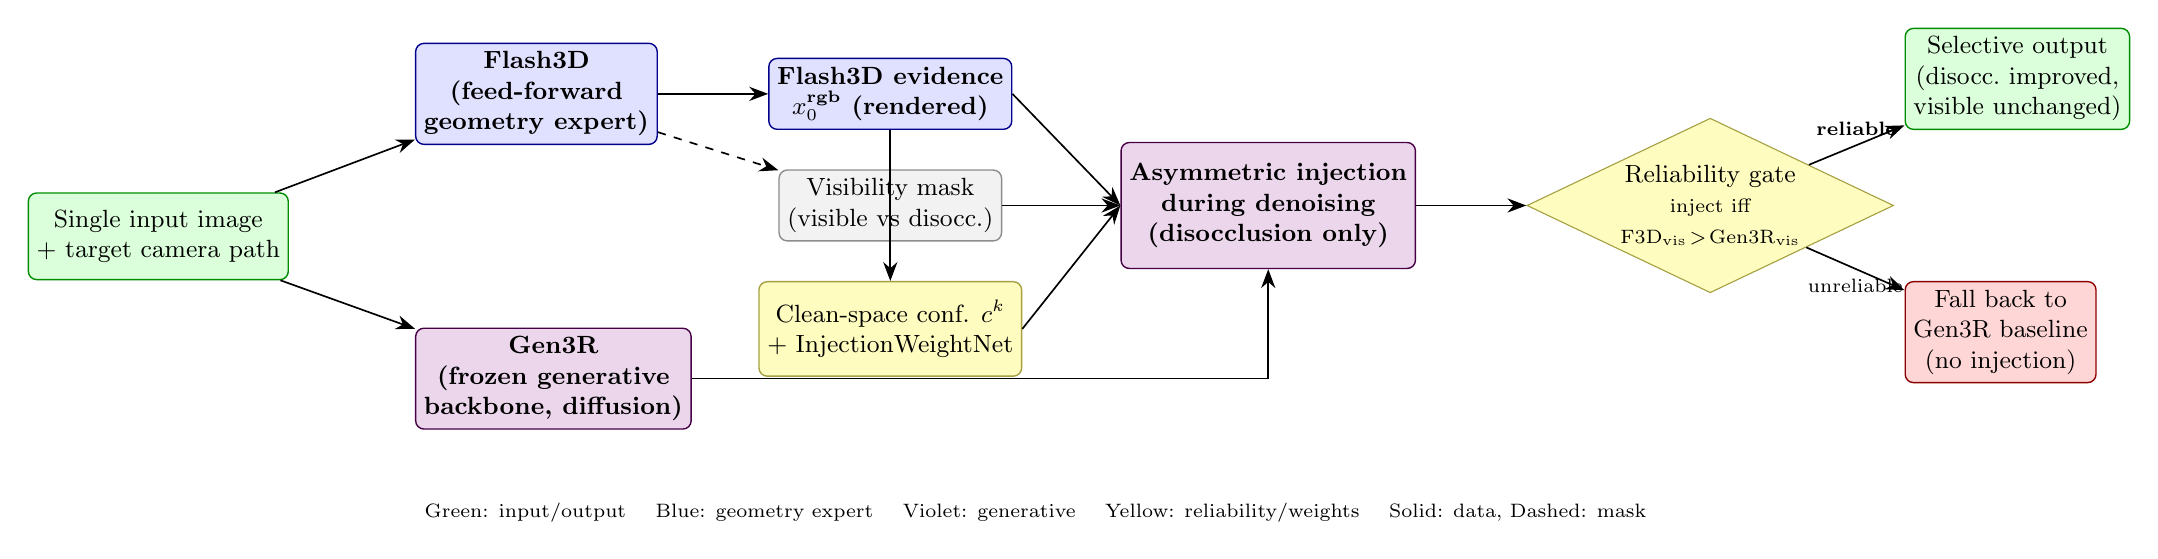
\begin{tikzpicture}[
  font=\small,
  >={Stealth[length=2.4mm]},
  node distance=7mm and 12mm,
  box/.style={rounded corners=3pt,draw,align=center,minimum height=11mm,minimum width=24mm,inner sep=3pt,line width=0.5pt},
  io/.style={box,fill=green!14,draw=green!55!black},
  geo/.style={box,fill=blue!12,draw=blue!55!black,font=\small\bfseries},
  gen/.style={box,fill=violet!16,draw=violet!55!black,font=\small\bfseries},
  aux/.style={box,fill=black!5,draw=black!45},
  wt/.style={box,fill=yellow!25,draw=yellow!60!black},
  neg/.style={box,fill=red!16,draw=red!55!black},
  gate/.style={diamond,aspect=2.1,draw,fill=yellow!25,draw=yellow!60!black,align=center,inner sep=1pt,minimum width=34mm},
  data/.style={->,line width=0.6pt},
  mask/.style={->,line width=0.6pt,dashed},
]

% column 1: input
\node[io] (input) {Single input image\\ + target camera path};

% column 2: two experts
\node[geo,above right=6mm and 16mm of input] (flash) {Flash3D\\ (feed-forward\\ geometry expert)};
\node[gen,below right=6mm and 16mm of input] (gen)   {Gen3R\\ (frozen generative\\ backbone, diffusion)};

% column 3: evidence / mask / conf
\node[geo,right=14mm of flash,minimum height=9mm] (ev)   {Flash3D evidence\\ $x_0^{\text{rgb}}$ (rendered)};
\node[aux,below=5mm of ev,minimum height=9mm]     (vm)   {Visibility mask\\ (visible vs disocc.)};
\node[wt,below=5mm of vm,minimum height=12mm]     (conf) {Clean-space conf. $c^k$\\ + InjectionWeightNet};

% column 4: injection
\node[gen,right=15mm of vm,minimum width=30mm,minimum height=16mm] (inj) {Asymmetric injection\\ during denoising\\ (disocclusion only)};

% column 5: gate
\node[gate,right=14mm of inj] (gate) {Reliability gate\\ \scriptsize inject iff\\ \scriptsize $\text{F3D}_{\text{vis}}\!>\!\text{Gen3R}_{\text{vis}}$};

% column 6: outputs
\node[io,above right=4mm and 13mm of gate] (outp) {Selective output\\ (disocc.\ improved,\\ visible unchanged)};
\node[neg,below right=4mm and 13mm of gate] (outn) {Fall back to\\ Gen3R baseline\\ (no injection)};

% edges
\draw[data] (input) -- (flash);
\draw[data] (input) -- (gen);
\draw[data] (flash) -- (ev);
\draw[mask] (flash) -- (vm);
\draw[data] (ev) -- (conf);
\draw[data] (ev.east) -- (inj.west);
\draw[data] (vm) -- (inj);
\draw[data] (conf.east) -- (inj.west);
\draw[data] (gen.east) -| ($(inj.south)+(0,-6mm)$) -- (inj.south);
\draw[data] (inj) -- (gate);
\draw[data] (gate) -- node[above,font=\scriptsize\bfseries]{reliable} (outp);
\draw[data] (gate) -- node[below,font=\scriptsize]{unreliable} (outn);

% legend
\node[font=\scriptsize,anchor=north west,align=left] at ($(gen.south west)+(0,-8mm)$)
  {Green: input/output \quad Blue: geometry expert \quad Violet: generative \quad Yellow: reliability/weights \quad Solid: data, Dashed: mask};

\end{tikzpicture}
\end{document}
